\chapter{Surface Simulations results}
\label{chap:ehd_res}

\section{Introduction}
In previous chapters, we established that {\ehd} better models the passivated surface and that we can achieve significant run time improvement using GPUs. In this section, we present the first results from the simulations. The chapter begins with an overview of prepossessing the output waveform, then shows how {\ehd} can match experimental data from the scanner. We then show how the model can be used to estimate the collection efficiency of {\onbb} events and finally create a simple background spectrum using them.

\section{Post-Processing}

In HPGe detector, adding a filter to the waveform can reduce the electronic noise and thus improve the energy resolution by averaging fluctuations in charge collection. We apply a trapezoidal filter to the pulse to match how the energy is picked off in experimental data in LEGEND. Fig. \ref{ch5_fig_trap_filter} shows how the waveform and trap filter output. Then the energy is picked off from a time on the flat top.

\begin{figure}%[!htb]
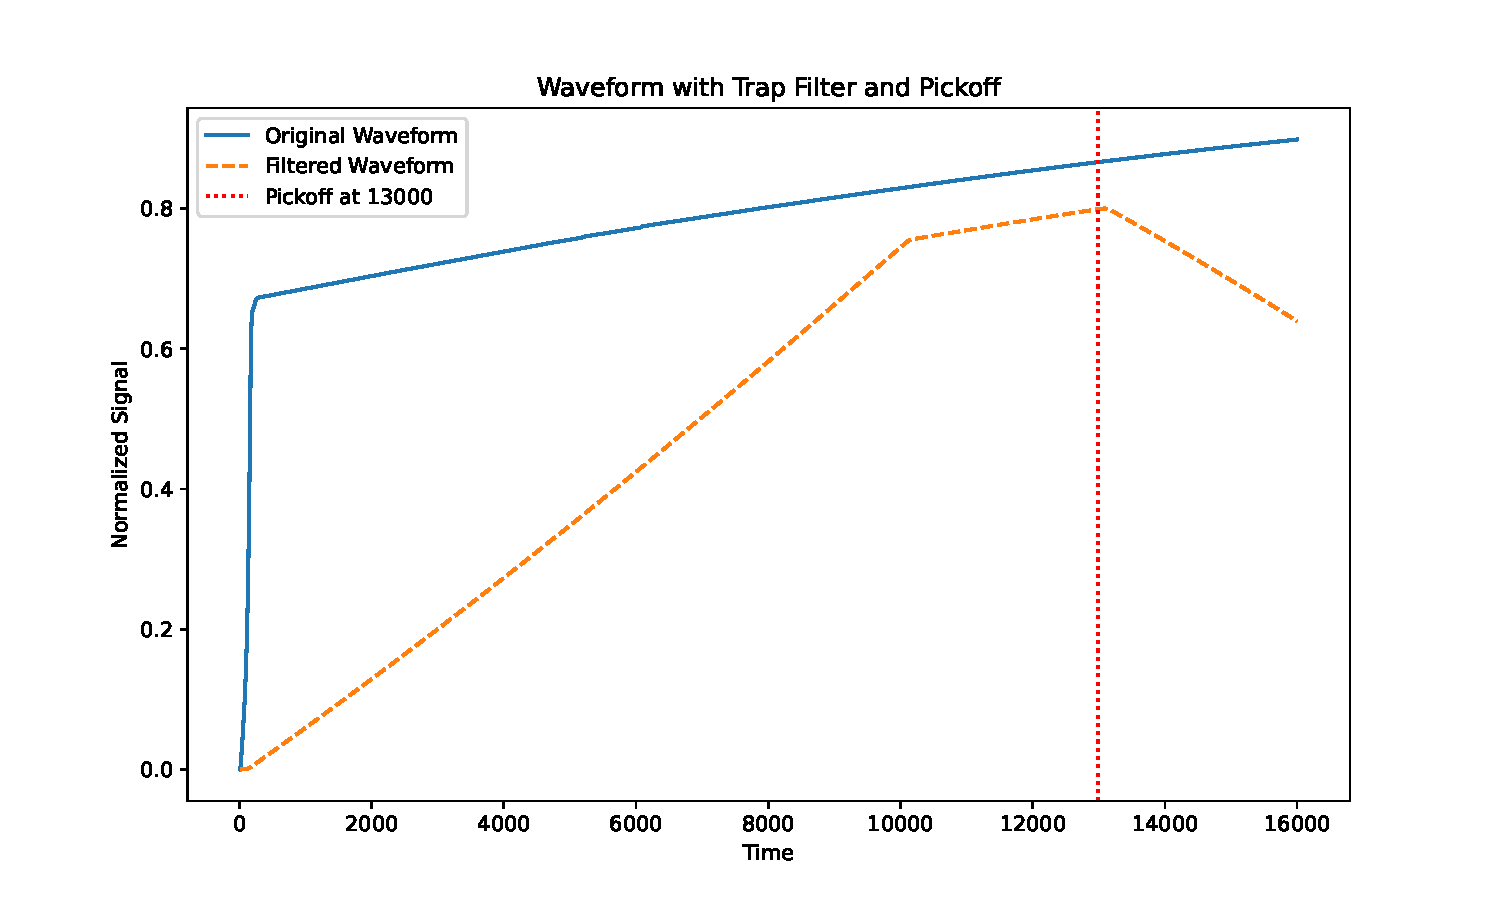
\includegraphics[trim={0cm 0cm 0cm 0cm},clip,width=0.9\linewidth]{ch5/figs/trap_filt.pdf}
\caption{Trap filter on highly degraded surface waveform. Filter had a rise time of 3000 ns, flat time of 2000 ns and the value was picked oof at 4000 ns.}
\label{ch5_fig_trap_filter}
\end{figure}

To understand the charge collection at different points on the detector, we map the detector using about 100 points, coarsely spaced, as shown in Fig. \ref{ch5_fig_activeness_points_neg}. These points can be used to generate an activeness map for a detector like Fig. \ref{ch5_fig_activeness_map_neg}. This map is produced by interpolating using cubic interpolation. The activeness map gives an understanding of how the charge collection efficiency works. Points at the same height but larger radii have lower activeness, as holes must travel a longer distance, increasing the likelihood of being pulled onto the surface by the negative surface charge. Since each event takes a few minutes to run, it is important to know the optimum number of events needed to sample the map enough for an interpolation. We estimate that about 100 points sampled in total in the r and z directions are enough.

\begin{figure}%[!htb]
%[trim={left bottom right top},clip]
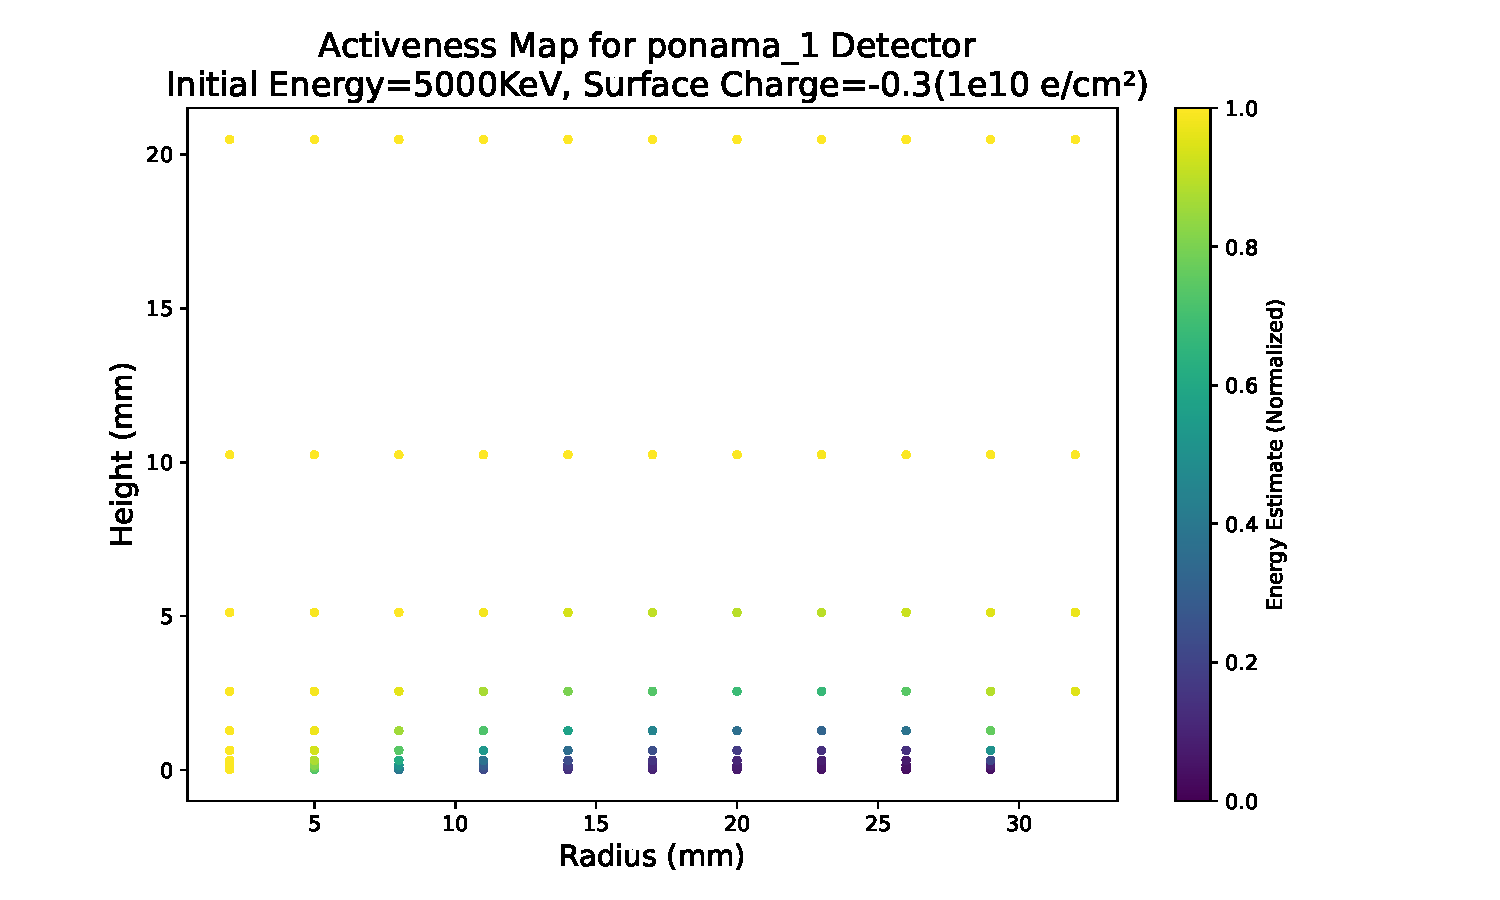
\includegraphics[trim={0cm 0.5cm 3.2cm 1.15cm},clip,width=0.9\linewidth]{ch5/figs/activenss_map_ponama_1_-0.3.pdf}
\caption{Activeness values to map a PPC detector \ehd with initial energy 5000 keV and negative surface charge. The radius points were uniformly spaced while the height points were densely sampled close to the surface.}
\label{ch5_fig_activeness_points_neg}
\end{figure}

\begin{figure}%[!htb]
%[trim={left bottom right top},clip]
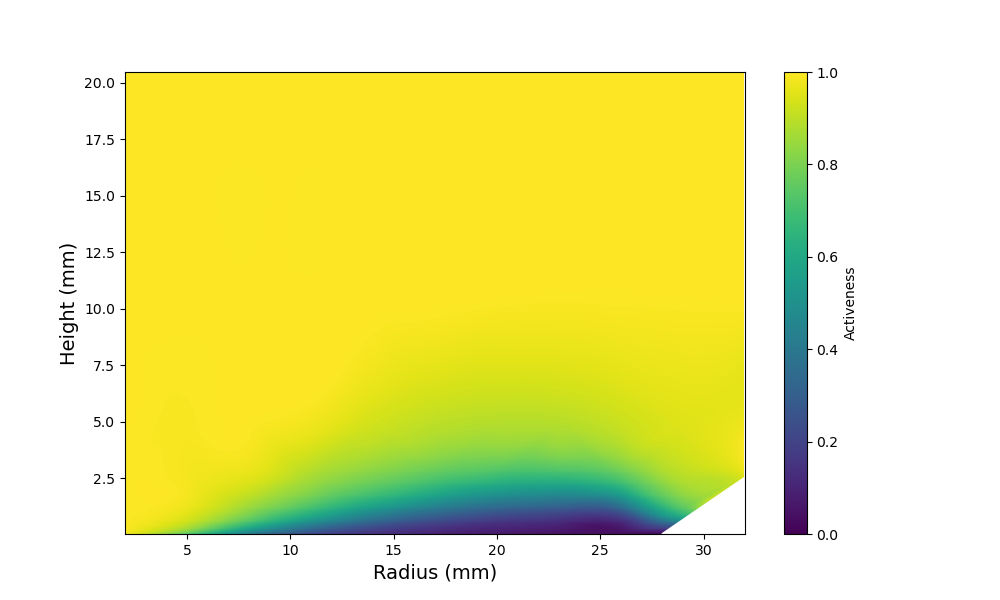
\includegraphics[trim={1.4cm 0.5cm 3.2cm 1.755cm},clip,width=0.9\linewidth]{ch5/figs/activeness_map_cubic_sc=-0.3_ponama_1_5000.png}
\caption{Interpolated activeness map for a PPC detector using \ehd with negative surface charge. Larger radius higher chance of hole component being pulled onto the surface causing higher loss of activeness.}
\label{ch5_fig_activeness_map_neg}
\end{figure}

Fig. \ref{ch5_fig_interpolated_activeness_map_0} illustrates the activeness maps without any surface charge. In this case, there is not much reduction in activeness. 

\begin{figure}%[!htb]
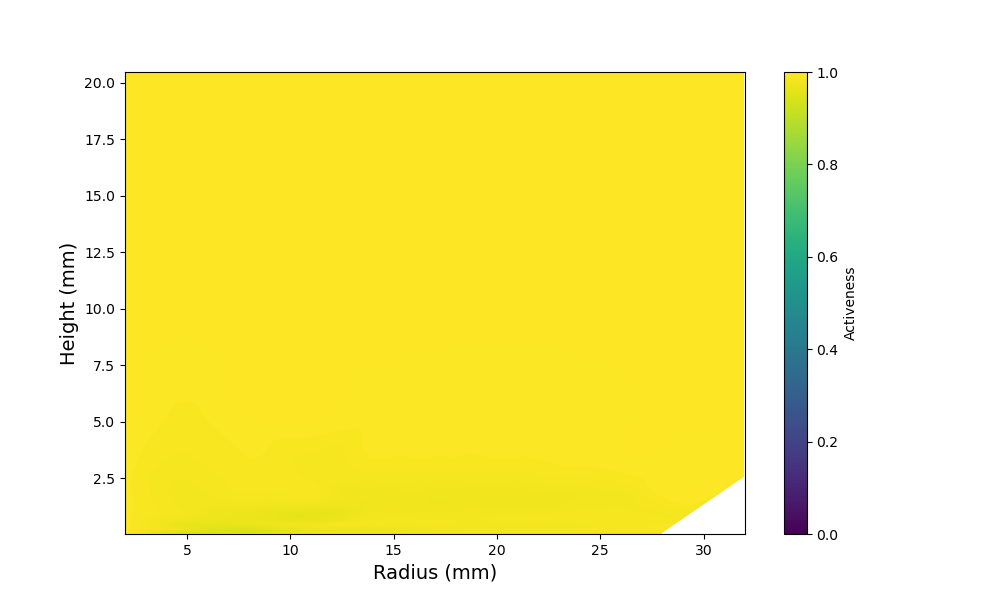
\includegraphics[trim={1.5cm 0cm 3.3cm 1cm},clip,width=0.9\linewidth]{ch5/figs/activeness_map_cubic_sc=0_ponama_1_5000.png}
\caption{Interpolated activeness map for a PPC detector using \ehd with zero positive surface charge. Without surface charge there is almost full collection.}
\label{ch5_fig_interpolated_activeness_map_0}
\end{figure}

Fig. \ref{ch5_fig_interpolated_activeness_map_pos} shows the activeness map for positive surface charge; points at the same height but lower radii have lower activeness, as electrons must travel a longer distance, increasing the likelihood of being pulled onto the surface by the negative surface charge. The activeness loss is less than that of negative surface charges since electrons are the minority charge carriers.

\begin{figure}%[!htb]
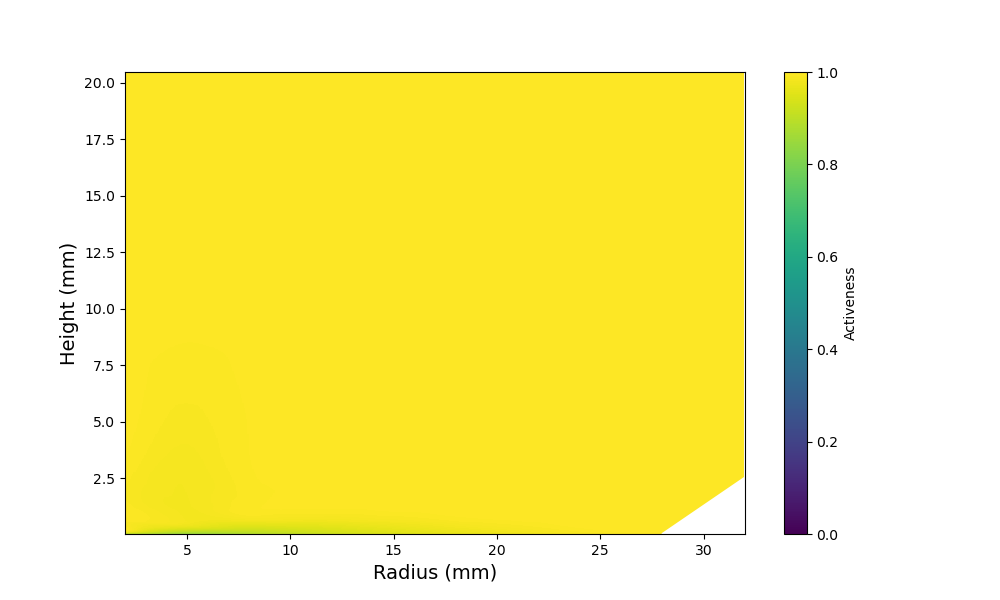
\includegraphics[trim={1.5cm 0cm 3.3cm 1cm},clip,width=0.9\linewidth]{ch5/figs/activeness_map_cubic_sc=0.3_ponama_1_5000.png}
\caption{Interpolated activeness map for a PPC detector using \ehd with positive surface charge. Lower radius higher chance of electron component being pulled onto the surface causing higher loss of activeness. The activeness loss is smaller than negative surface charge since electrons are minority signal component.}
\label{ch5_fig_interpolated_activeness_map_pos}
\end{figure}


\section{\label{res:1} Reproduction of Results from Established Test Stands}

To validate EH-Drift against existing measurements, we modeled alpha events studied by TUBE and  GALATEA  scanning test stands. We simulated the events in {\ponama} (PPC from ORTEC made from Natural Material) detector. This was a natural Germanium detector that was made similar to PPC detectors used in {\MJD}. We simulated events using various surface charges and surface drift speeds.  We then fit those different curves to data to estimate the amount of surface charge present to show such behavior.

%We generated 8$\mu$s pulse using {\ehd} and applied a trap filter of 4$\mu$s rise time, 3$\mu$s flat-top time, and picked off energy at 7$\mu$s.
\begin{figure}%[!htb]
%[trim={left bottom right top},clip]
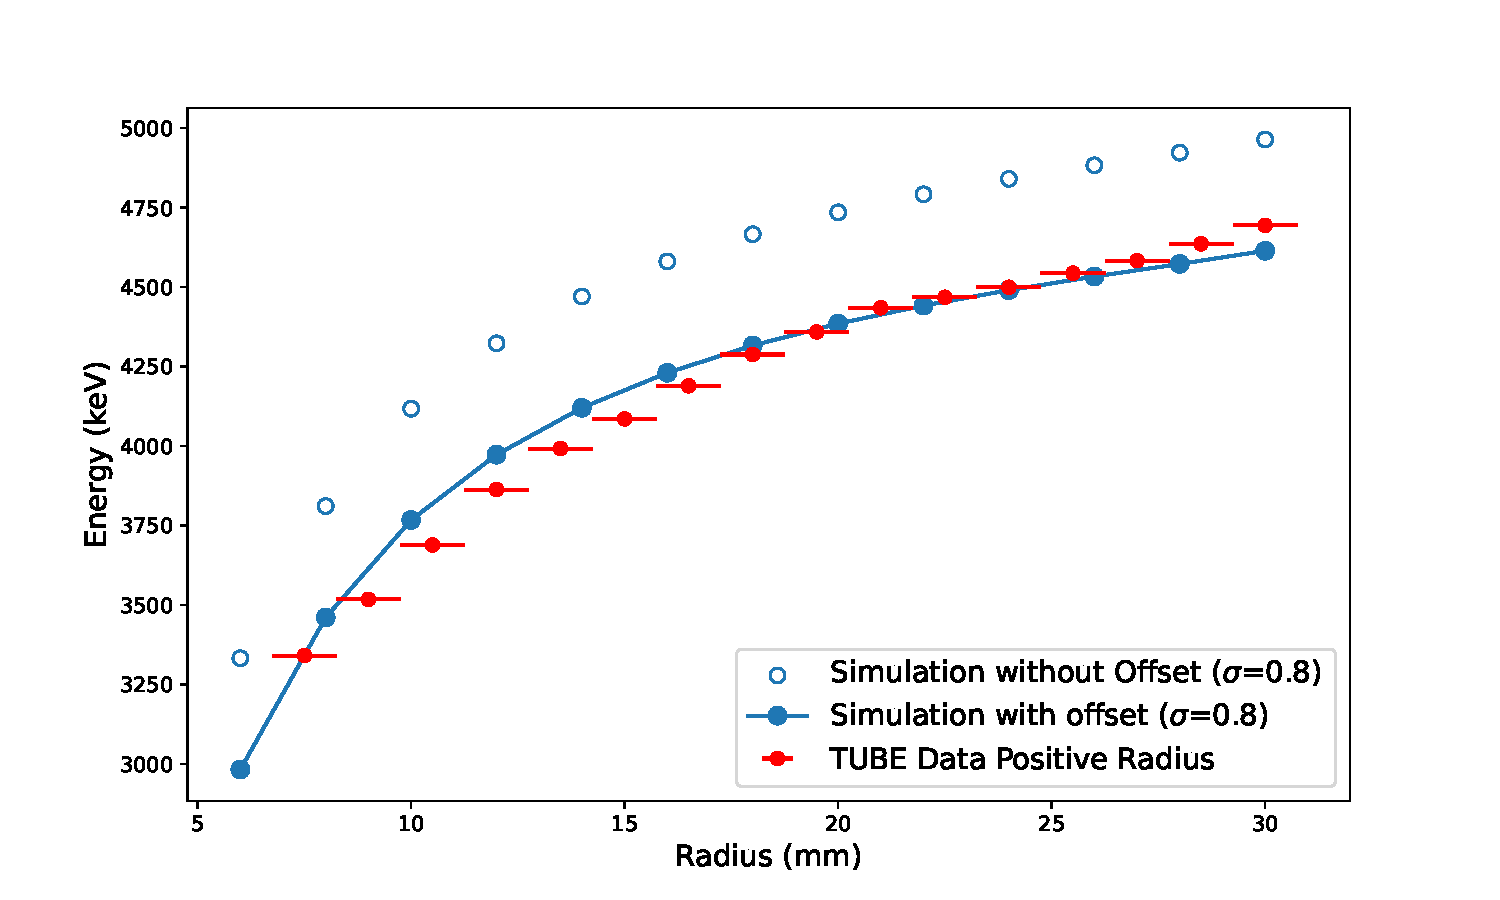
\includegraphics[trim={0.3cm 0.1cm 1.7cm 0.1cm},clip,width=\linewidth]{ch5/figs/tube_fit.pdf}
\caption{Fitting the activeness in TUBE scanner with \ehd{}.}
\label{fig:tube_fit}
\end{figure}


\begin{figure}%[!htb]
%[trim={left bottom right top},clip]
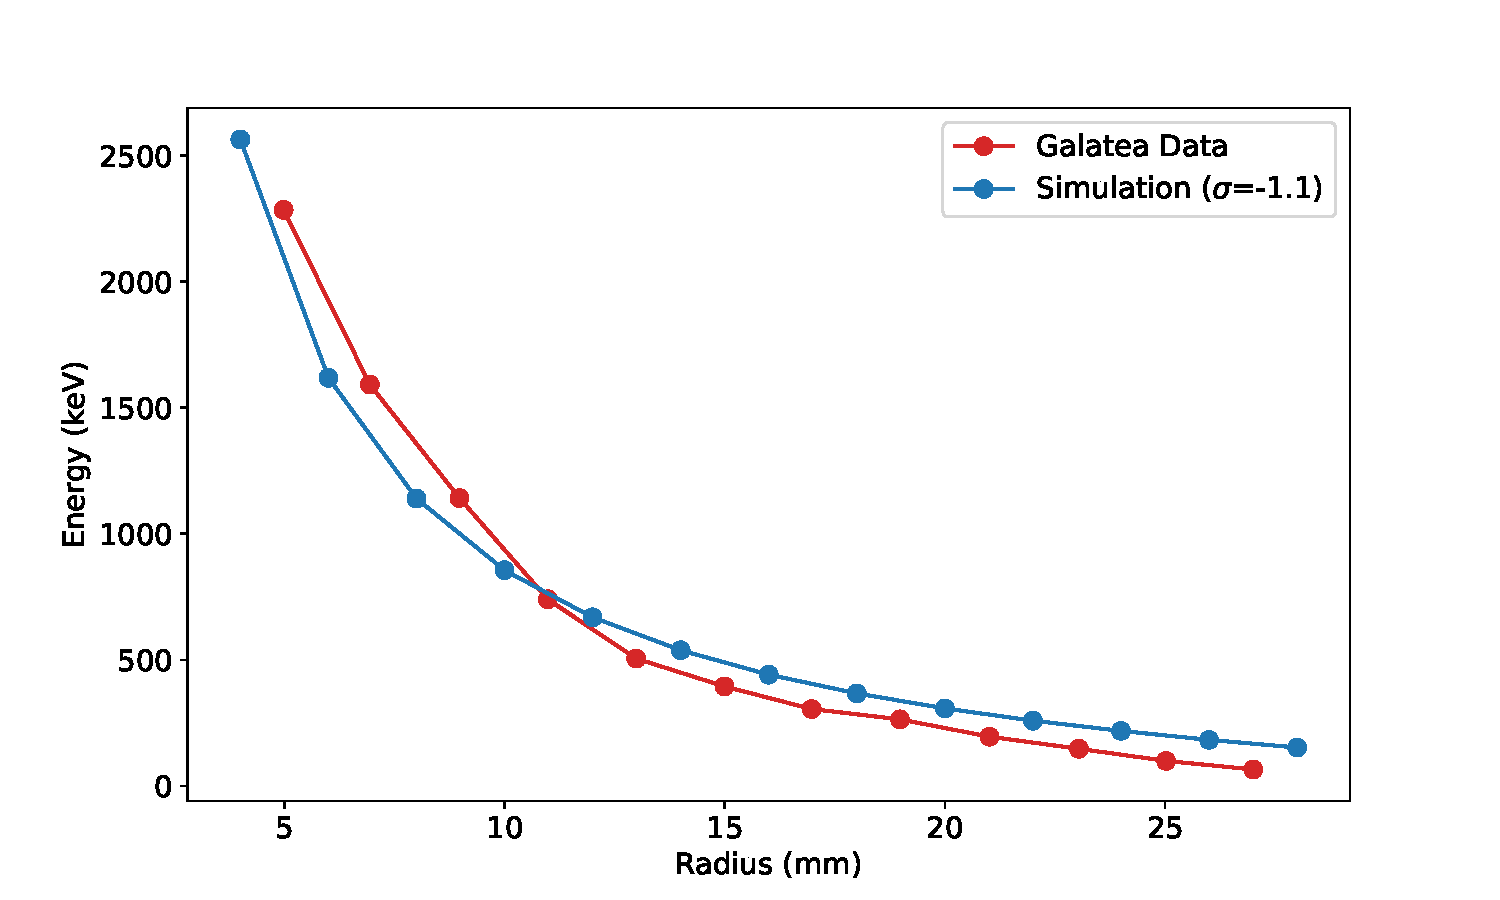
\includegraphics[trim={0.3cm 0.1cm 1.7cm 1cm},clip,width=\linewidth]{ch5/figs/gal_fit.pdf}
\caption{Fitting the activeness in GALATEA scanner with \ehd{}.}
\label{fig:gal_fit}
\end{figure}

We found a positive surface charge explains the behavior observed in TUBE. Fig. \ref{fig:tube_fit} compares TUBE scanner data to EH-Drift simulations with a positive surface charge. Positive surface charge would attract electrons on the surface, which would result in energy degradation. In this scenario, electrons are collected at the n+ surface, so the closer the points are to the origin, the more chance there is for the electrons to get trapped onto the surface, and the more energy degradation there is. Thus, collected energy is proportional to radius. While the simulations have matched the trend well, there appears to be an offset. This could be because the source beam used in TUBE had about $0.75$ mm uncertainty in position. There could also be a dead region before the passivated surface. We added an energy offset to account for this offset.

In the GALATEA scanner, the behavior can be explained using a negative surface charge as shown in Fig. \ref{fig:gal_fit}. Negative surface attracts holes to the surface and since holes are collected at the point contact, located at r=0, the higher the radius, more charges end up on the surface. Thus, collected energy falls inversely with radius.

\section{\label{res:2} Estimating efficiency in ROI}

We can use the maps created by EH to estimate the collections efficiency of signature events such as {\onbb}. Experiments such as Legend have a region of interest (ROI) band determined by the energy resolutions of the detector. ROI is used to classify if an event is a signature event or not; however, if the event happens close to the surface, there is a chance that the collected energy would be degraded enough to not register as an event in ROI. To understand this effect, we created activeness maps for detectors with 2039 keV initial energy for various surface charges. We then randomly sample points uniformly in the detector and estimate their activeness using the interpolated map. A 3 keV threshold is defined for the Region of Interest (ROI), meaning that if the activeness at a point falls below 3 keV, that event is not registered as a {\onbb} event. Each point is assigned a value of 1 if it is counted as {\onbb}, or 0 otherwise. Fig.\ref{ch5_fig_binary_activenss} shows this binary activeness for a PPC detector with negative surface charge. The overall efficiency is then calculated as the sum of activeness values divided by the total number of points, while also factoring in the phi dependence.

\begin{figure}%[!htb]
\centering
%[trim={left bottom right top},clip]
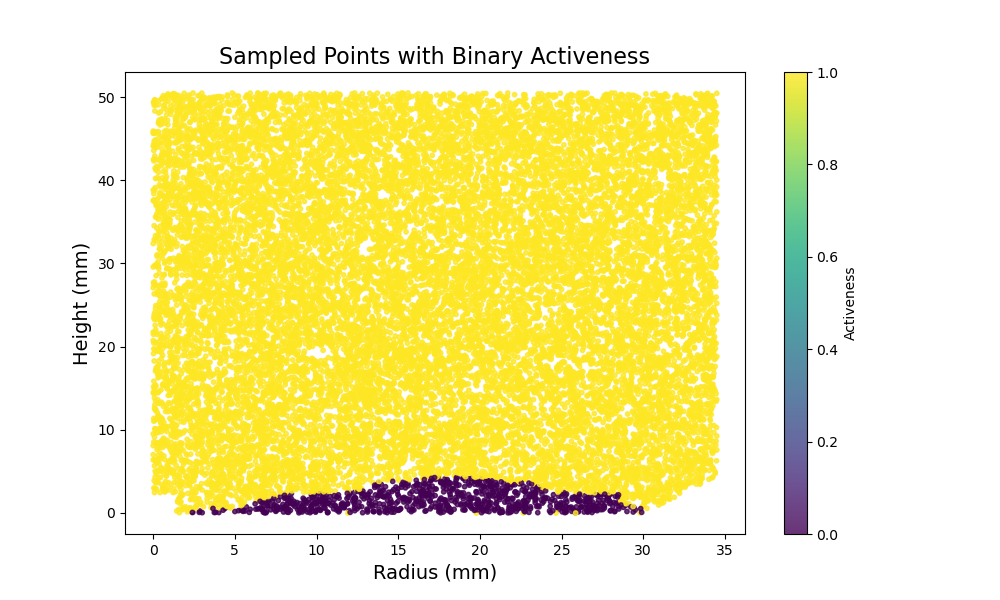
\includegraphics[trim={1.5cm 0cm 6cm 1.77cm},clip,width=0.9\linewidth]{ch5/figs/bianry_act_ponama_1_-0.03.png}
\caption{Binary activeness for {\ponama} detector with negative surface charge. A $3$ keV energy resolution threshold is defined. If energy is degraded above it, it is labeled zero, else 1. The blue dots show where {\onbb} events would be not be recorded for this detector.}
\label{ch5_fig_binary_activenss}
\end{figure}

Fig. \ref{fig:efficiency_sc_plot} shows the estimated efficiency versus surface charge for the {\ponama} detector, a LEGEND PPC detector, and a LEGEND ICPC detector. The efficiency drops rapidly for negative surface charges in both PPC detectors; however, it decreases most sharply for {\ponama}, which has a lower depletion voltage and thus a weaker electric field near the surface. The LEGEND PPC detector also loses efficiency quickly because of its larger passivated surface, but its higher electric field moderates the overall loss more than in {\ponama}.

\begin{figure}%[!htb]
%[trim={left bottom right top},clip]
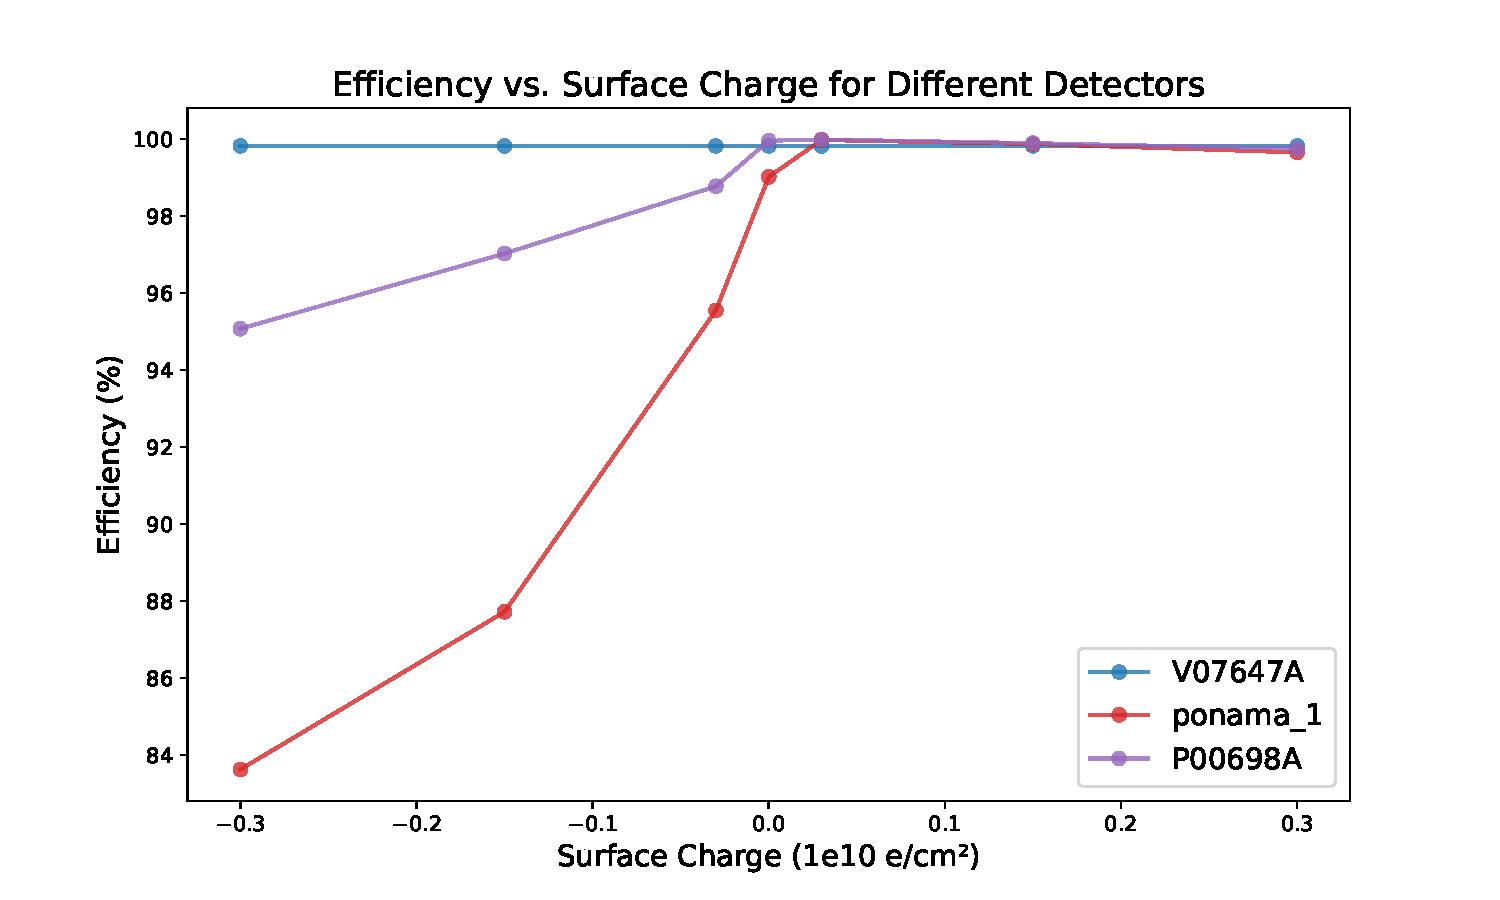
\includegraphics[trim={1.6cm 0.3cm 2cm 1.8cm},clip,width=\linewidth]{ch5/figs/efficiency_0nbb.pdf}
\caption{Efficiency in the ROI versus surface charge.}
\label{fig:efficiency_sc_plot}
\end{figure}

The Mirion-style ICPC detector exhibits virtually no reduction in activeness, primarily because it has a much smaller passivated surface. The collection efficiency is $99.82\%$. To understand this slight reduction in efficiency, one can look at the electric field at the ditch of the detector shown in Fig. \ref{ch5_fig_elect_field_lines_surface_V07647A}. The field lines indicate that the electron components near the surface will be pulled onto the ditch which is passivated. This loss in activeness is much smaller than in other types of detectors. Since LEGEND-1000 plans to use Mirion-style ICPC detectors, surface backgrounds in that experiment are expected to be significantly reduced.

\begin{figure}%[!htb]
%[trim={left bottom right top},clip]
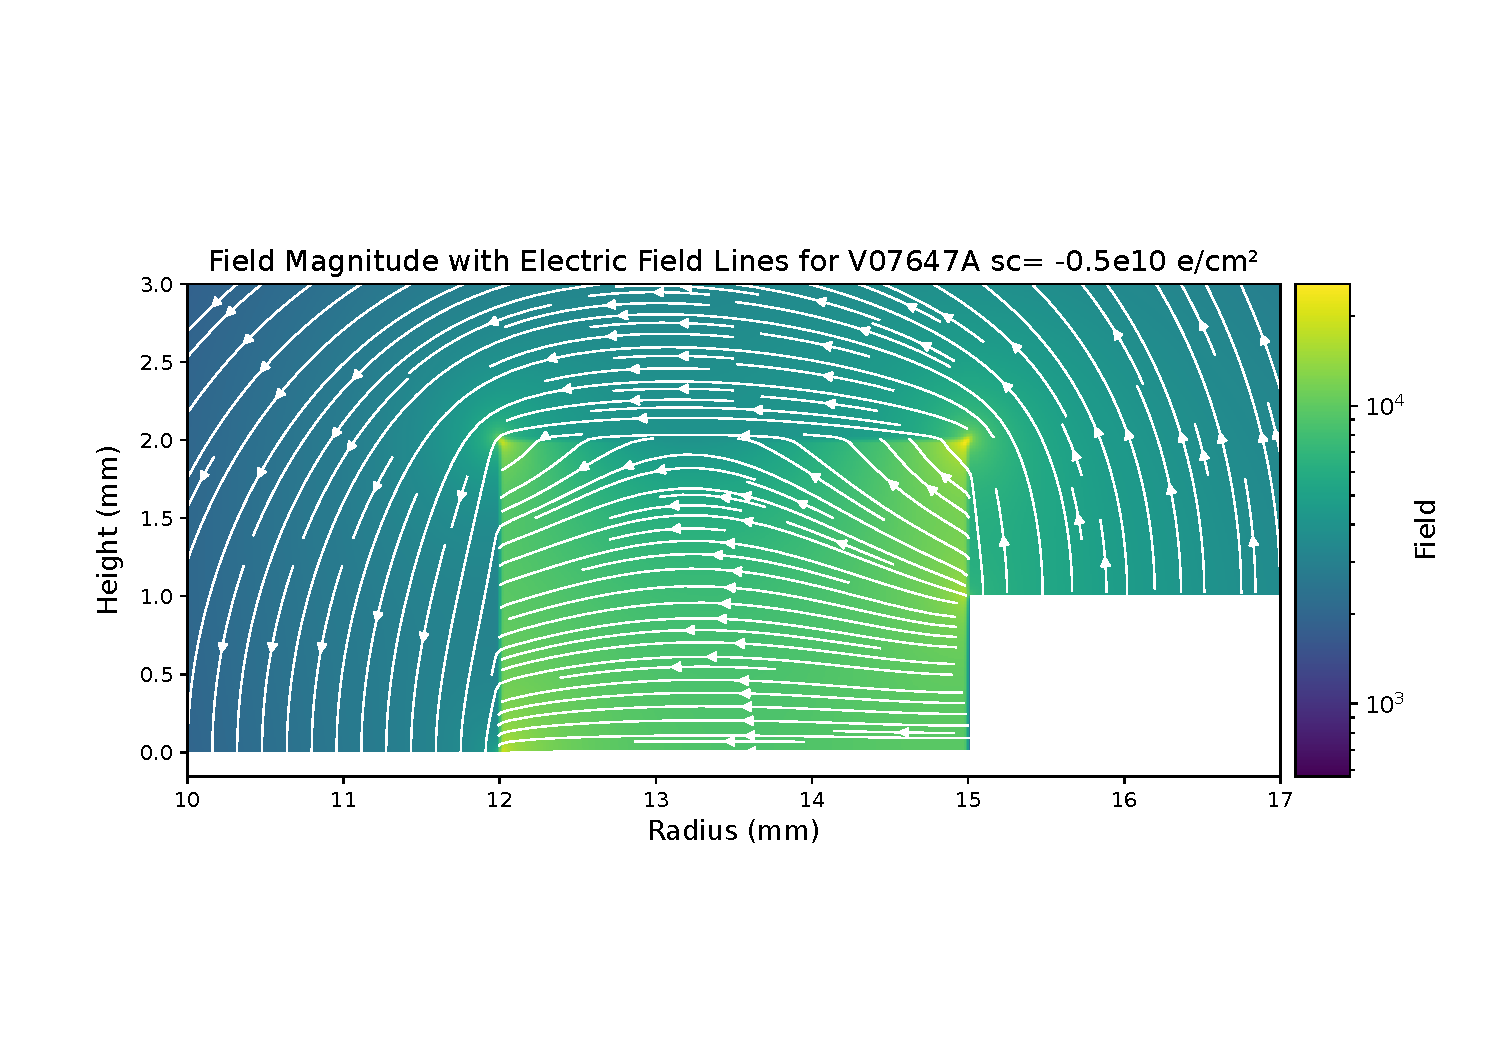
\includegraphics[trim={0cm 3cm 0cm 4.69cm},clip,width=0.99\linewidth]{ch5/figs/elect_field_lines_surface_V07647A_sc_-0.5.pdf}
\caption{Electric magnitude and field lines near the ditch of a Mirion ICPC detector with negative surface charge. The field lines attract electron component to the surface which drift slowly. The reduction in activeness is fraction of other dector geometries.}
\label{ch5_fig_elect_field_lines_surface_V07647A}
\end{figure}


\section{\label{res:3} Generating Background Spectra}

Geant4 is a Monte Carlo-based toolkit that can simulate the passage of particles through matter. To demonstrate how EH-Drift can be used to create a background model, we performed a {\geant} simulation of a germanium detector exposed to a planar 5\,MeV alpha source. We recorded the resulting hits from alpha particles entering the detector. We then used the activeness map to estimate the energy that would be collected due to surface effects. Fig. \ref{fig:eng_spec_degradation} how the collected energy spectrum would look like for various surface charge scenarios. Notably, the spectrum for negative surface charge closely matches alpha spectra estimated in experimental data.

\begin{figure}%[!htb]
  \centering
      %[trim={left bottom right top},clip]
  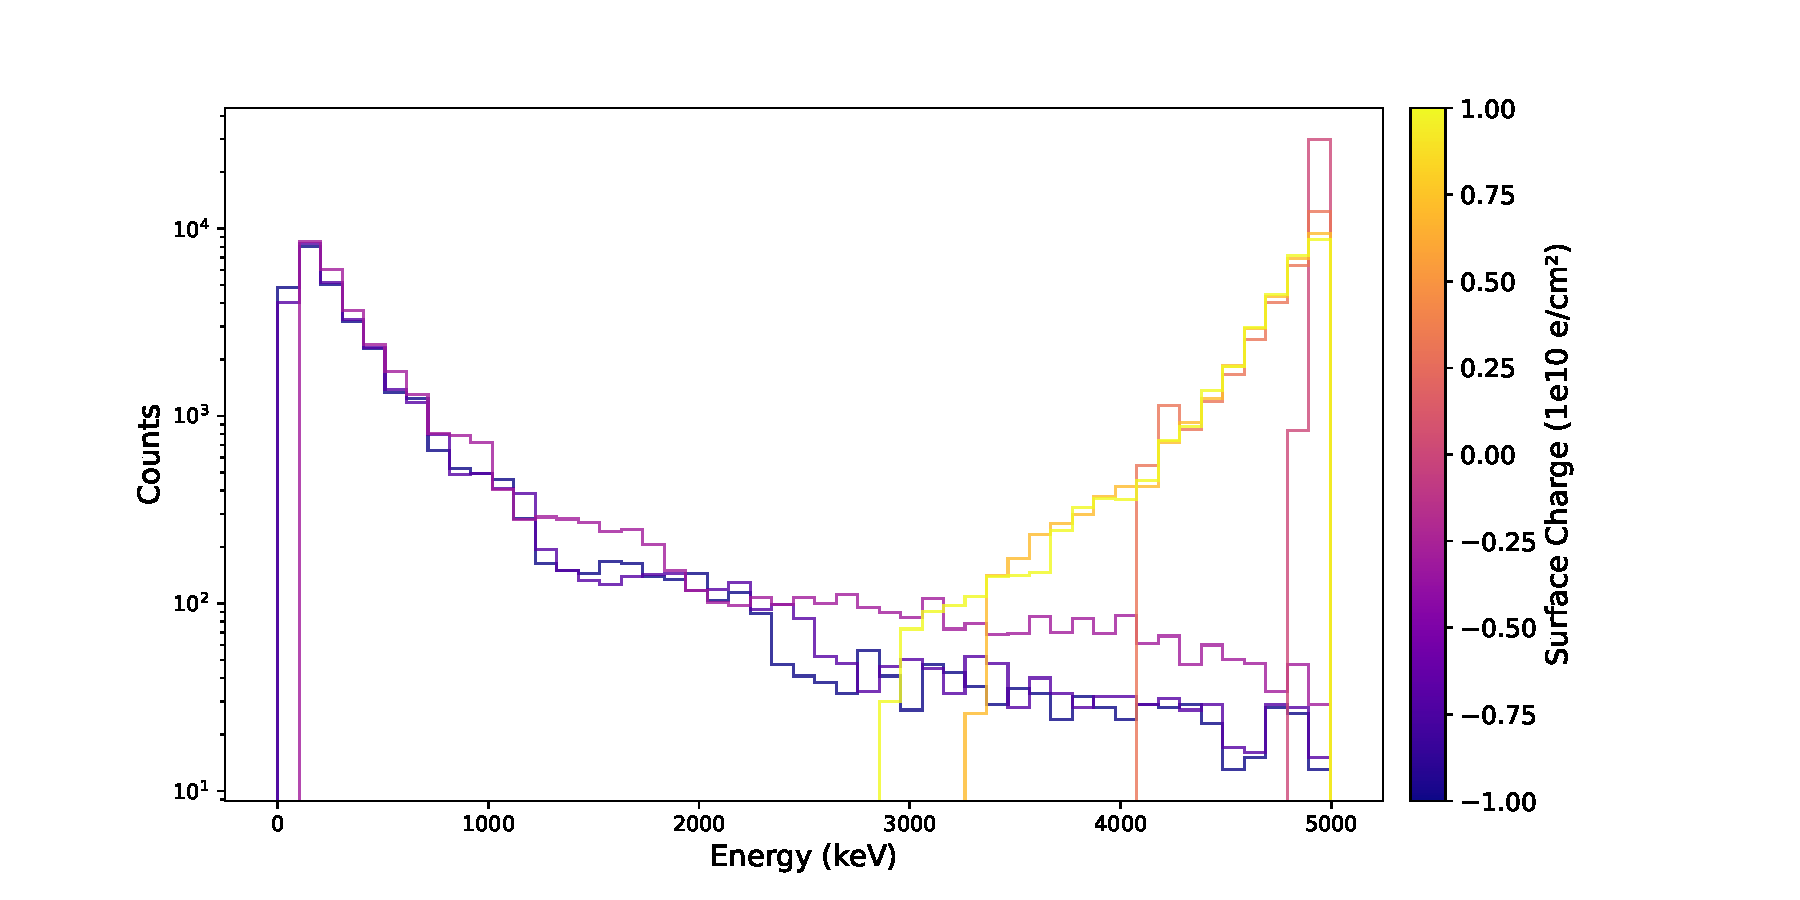
\includegraphics[trim={2cm 0.5cm 4.5cm 1.7cm},clip,width=0.99\linewidth]{ch5/figs/eng_deg_hist.pdf}
  \caption{Degradation of the alpha-particle energy spectrum under various surface charges. The initial alpha energy was 5\,MeV.}
  \label{fig:eng_spec_degradation}
\end{figure}

To understand the effect of passivated surface on Beta particles, we simulated the spectrum of K$^{42}$ using {\geant}. The output energy spectrum is shown by the blue histogram in Fig.\ref{ch5_figs_k_42_degrad}. The spectrum has a prominent gamma line at 1500 keV and a broad beta continuum extending to 3500 keV, which is the Q-value of the decay. Using {\ehd} we estimated the activeness of the passivated surface assuming $2039$ keV energy map. The resulting spectrum is shown by the yellow curve.

\begin{figure}%[!htb]
  \centering
      %[trim={left bottom right top},clip]
  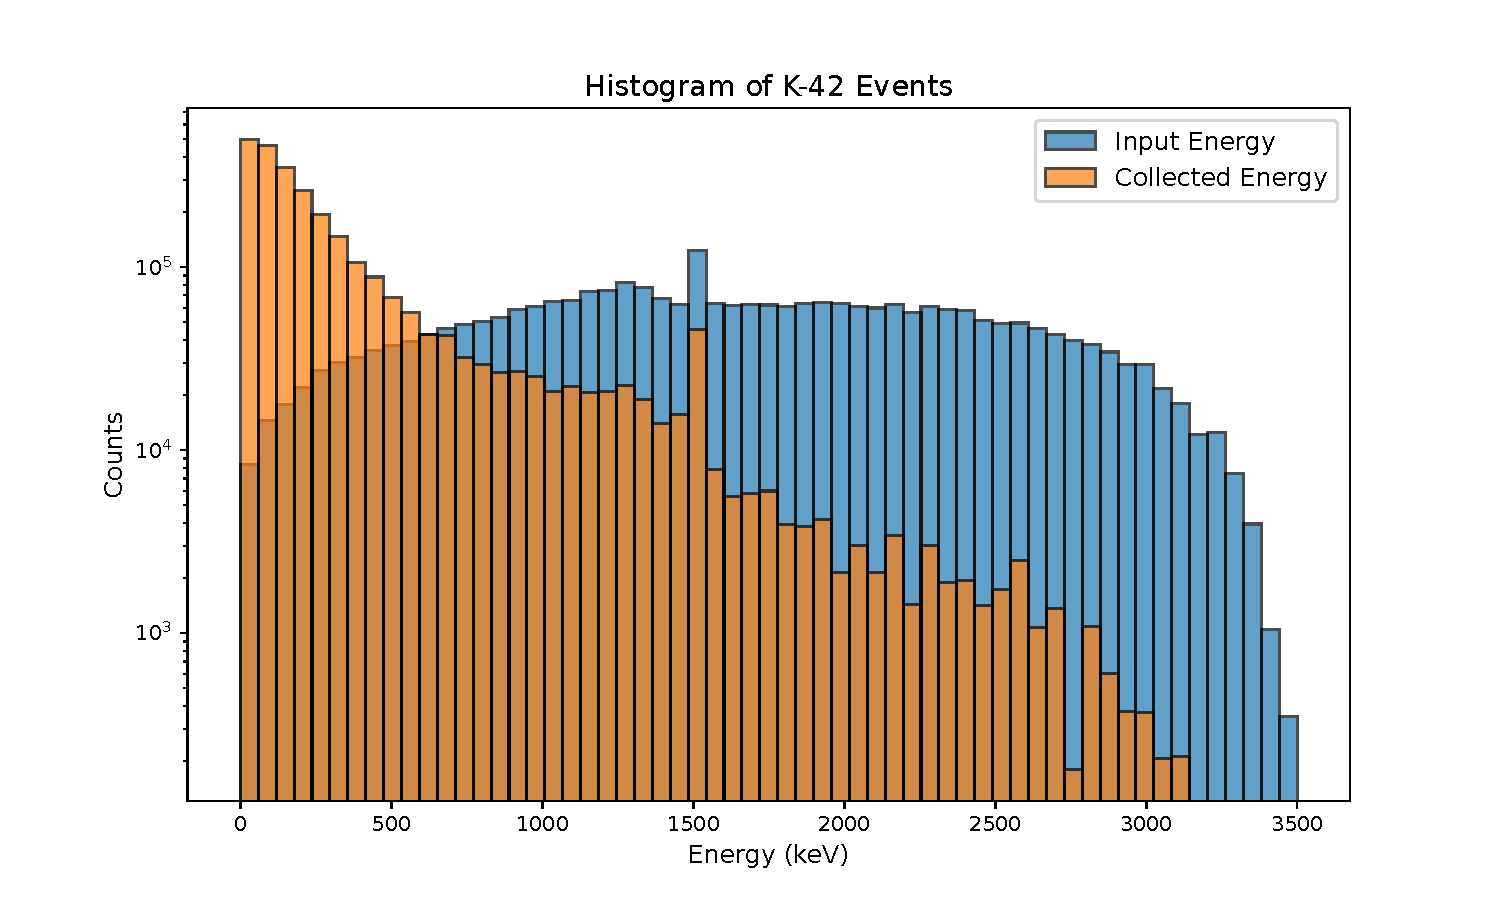
\includegraphics[trim={1.5cm 0.0cm 2cm 1.76cm},clip,width=0.99\linewidth]{ch5/figs/k_42_beta_spectrum.pdf}
  \caption{Degradation of the K-42 energy spectrum in {\ponama} detector. The detector surface had a surface charge of $- 0.5 \times 10^{-10} \frac{e}{cm^2}$. The activeness was calculated assuming $2039$ keV energy map. Curve does not model dead layer in Lithium n$^+$ contact.}
  \label{ch5_figs_k_42_degrad}
\end{figure}

